% !TeX spellcheck = en_US
\addscenariosection{1}{Gameplay}{AI evolutionary}{\images/ai_pawn.png}
 
\textbf{Author:} Invoceusse and Philenarion

For use this AI, choose a faction for it.\\
\\

The AI use 4 decks:
\begin{itemize}
    \item Unit (The units used in battle)
    \item Ability (The Abilities the AI may know, each time an AI Hero card "Use a skill" is played: draw a card from this deck. Shuffle it only at start of battle)
    \item Spell (The spells the AI may know, each time an AI Hero card "Cast a spell" is played: draw a card from this deck. Shuffle it only at start of battle)
    \item AI Hero cards (The deck used by the AI, see 33 of the rulebook)
\end{itemize}


The spell and ability decks are bigger than the AI hero cards deck so the player doesn't know which spell/ability is cast. \\
Don’t forget to shuffle all decks before the battle.\\
\\

This AI is designed with a map with these starting conditions:

\textbf{Starting Resources:} 5 \svg{gold}, 2 \svg{building_materials}, 0 \svg{valuables}

\textbf{Starting Income:} 10 \svg{gold}, 0 \svg{building_materials}, 1 \svg{valuables}

\textbf{Starting Units:}
\begin{itemize}
    \item A Few \svg{silver} units of your choice.
\end{itemize}

\textbf{Town Buildings:} City hall

With other starting conditions the AI can be easier to kill. 

\newpage

\hommtable[]{40}{
    \centering
    \textbf{composition of AI decks}\\
    \centering
    
    \newcommand{\bronze}[0]{\svg[12]{bronze}}
    \newcommand{\silver}[0]{\svg[12]{silver}}
    \newcommand{\golden}[0]{\svg[12]{golden}}
    \newcommand{\azure}[0]{\svg[12]{azure}}
    
    \begin{tabularx}{\linewidth}{p{0.15\linewidth}XXXX} & \darkcell{Unit AI} & \darkcell{Spells AI} & \darkcell{AI ability} & \darkcell{AI Hero cards }\\
        \darkcell[1.2]{turn 1}
        & \lightcell[1.2]{1 few \silver}
        & \lightcell[1.2]{add 1 magic arrow.\footref{azure}}
        & \lightcell[1.2]{No one at this time}
        & \lightcell[1.2]{3 Might cards.\\
                          1 Magic card.}\\
        \darkcell[1.8]{turn 2}
            & \lightcell[1.8]{2 few \bronze \\ 1 few \silver}
            & \lightcell[1.8]{same as turn 1}
            & \lightcell[1.8]{add \textbf{2} new abilities.}
            & \lightcell[1.8]{3 Might cards.\\
                1 Skill card.\\
                1 Magic card.}\\
        \darkcell[1.8]{turn 3}
            & \lightcell[1.8]{3 few \bronze \\ 1 few \silver}
            & \lightcell[1.8]{same as turn 1}
            & \lightcell[1.8]{No more ability (\textbf{2} at this point).}
            & \lightcell[1.8]{3 Might cards.\\
                1 Skill card.\\
                1 Magic card.}\\

        \darkcell[1.8]{turn 4}
            & \lightcell[1.8]{3 few \bronze \\ 2 few \silver}
            & \lightcell[1.8]{same as turn 1}
            & \lightcell[1.8]{No more ability (\textbf{2} at this point).}
            & \lightcell[1.8]{4 Might cards.\\
                1 Skill card.\\
                1 Magic card.}\\
        \darkcell[1.8]{turn 5}
            & \lightcell[1.8]{3 few \bronze \\ 2 few \silver}
            & \lightcell[1.8]{Add \textbf{5} spells (don't forget starting spell \footref{azure}\footref{azure}.}
            & \lightcell[1.8]{No more ability (\textbf{2} at this point).}
            & \lightcell[1.8]{4 Might cards.\\
                1 Skill card.\\
                3 Magic card.}\\
        \darkcell[1.8]{turn 6}
            & \lightcell[1.8]{3 few \bronze \\ 2 few \silver}
            & \lightcell[1.8]{No more spell (\textbf{5} at this point + starting spell).}
            & \lightcell[1.8]{add \textbf{1} new abilitiy (\textbf{3} at this point).}
            & \lightcell[1.8]{4 Might cards.\\
                2 Skill card.\\
                3 Magic card.}\\
        
        
        \darkcell[1.8]{turn 7}
            & \lightcell[1.8]{1 few + 2 pack \bronze \\ 1 few + 1 pack \silver \\ Add wall/tower.}
            & \lightcell[1.8]{No more spell (\textbf{5} at this point + starting spell).}
            & \lightcell[1.8]{No more ability (\textbf{3} at this point).}
            & \lightcell[1.8]{4 Might cards.\\
                2 Skill card.\\
                3 Magic card.}\\
        \darkcell[1.8]{turn 8}
            & \lightcell[1.8]{1 few + 2 pack \bronze \\ 2 pack \silver \\ Add wall/tower.}
            & \lightcell[1.8]{No more spell (\textbf{5} at this point + starting spell).}
            & \lightcell[1.8]{add \textbf{2} new abilities (\textbf{5} at this point).}
            & \lightcell[1.8]{4 Might cards.\\
                3 Skill card.\\
                3 Magic card.}\\
        \darkcell[2.4]{turn 9}
            & \lightcell[2.4]{1 pack \bronze \\ 2 pack \silver \\ 2 few \golden \\ Add wall/tower.}
            & \lightcell[2.4]{Add \textbf{2} spells (\textbf{7} at this point + starting spell).}
            & \lightcell[2.4]{No more ability (\textbf{5} at this point).}
            & \lightcell[2.4]{4 Might cards.\\
                3 Skill card.\\
                4 Magic card.}\\
    \end{tabularx}
}


\footnotetext[1]{In easy add Earthquake. In normal add a second magic arrow.}
\footnotetext[7]{In impossible, in turn 5 and after, remove one magic arrow.}

\hommtable[]{25}{
    \centering
    \textbf{composition of AI decks}\\
    \centering
    
    \newcommand{\bronze}[0]{\svg[12]{bronze}}
    \newcommand{\silver}[0]{\svg[12]{silver}}
    \newcommand{\golden}[0]{\svg[12]{golden}}
    \newcommand{\azure}[0]{\svg[12]{azure}}
    
    \begin{tabularx}{\linewidth}{p{0.15\linewidth}XXXX} & \darkcell{Unit AI} & \darkcell{Spells AI} & \darkcell{AI ability} & \darkcell{AI Hero cards }\\
        \darkcell[2.4]{turn 10}
            & \lightcell[2.4]{1 pack \bronze \\ 2 pack \silver \\ 2 few \golden \\ Add wall/tower.}
            & \lightcell[2.4]{No more spell (\textbf{7} at this point + starting spell).}
            & \lightcell[2.4]{No more ability (\textbf{5} at this point).}
            & \lightcell[2.4]{5 Might cards.\\
                3 Skill card.\\
                4 Magic card.}\\
        \darkcell[2.4]{turn 11}
            & \lightcell[2.4]{1 pack \bronze \\ 2 pack \silver \\ 1 few + 1 pack \golden \\ Add wall/tower.}
            & \lightcell[2.4]{No more spell (\textbf{7} at this point + starting spell).}
            & \lightcell[2.4]{add \textbf{1} new abilities (\textbf{6} at this point).}
            & \lightcell[2.4]{5 Might cards.\\
                4 Skill card.\\
                4 Magic card.}\\
        \darkcell[2.4]{turn 12}
            & \lightcell[2.4]{1 pack \bronze \\ 2 pack \silver \\ 2 pack \golden \\ Add wall/tower.}
            & \lightcell[2.4]{Add \textbf{1} spells (\textbf{8} at this point + starting spell).}
            & \lightcell[2.4]{No more ability (\textbf{6} at this point).}
            & \lightcell[2.4]{5 Might cards.\\
                4 Skill card.\\
                5 Magic card.}\\
        \darkcell[2.4]{turn 13}
            & \lightcell[2.4]{2 pack \silver \\ 2 pack \golden \\ 1 neutral \azure \\ Add wall/tower.}
            & \lightcell[2.4]{No more spell (\textbf{8} at this point + starting spell).}
            & \lightcell[2.4]{No more ability (\textbf{6} at this point).}
            & \lightcell[2.4]{5 Might cards.\\
                4 Skill card.\\
                5 Magic card.}\\
    \end{tabularx}
}
\\
\subsection*{\MakeUppercase{Skill list AI}}
When AI adds abilities in his deck, draw cards until you draw one of the abilities in the following lists, discard the other cards in the same order they were drawn: 
Air magic / Archery / Armorer / Artillery / Earth magic / Fire magic / First aid / Offense / Resistance / Sorcery / Water Magic. 
\begin{center}
    
\includegraphics[width=0.1\paperwidth]{\_assets/ai/skill/skill_1.png}
    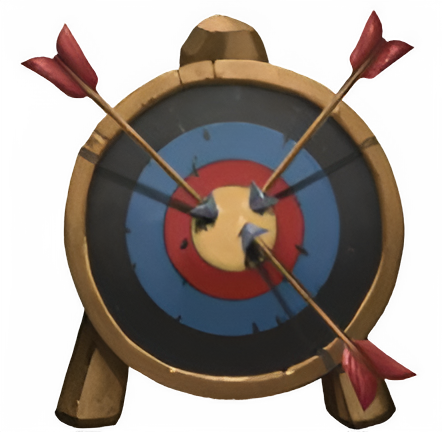
\includegraphics[width=0.1\paperwidth]{\_assets/ai/skill/skill_2.png}
    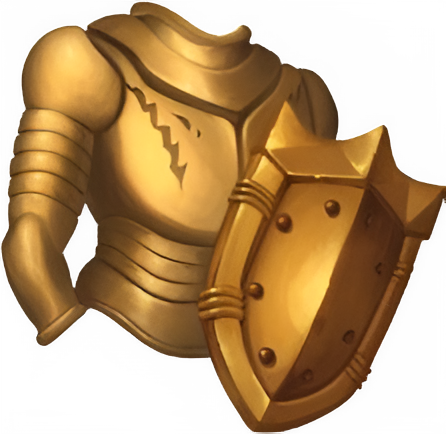
\includegraphics[width=0.1\paperwidth]{\_assets/ai/skill/skill_3.png}
    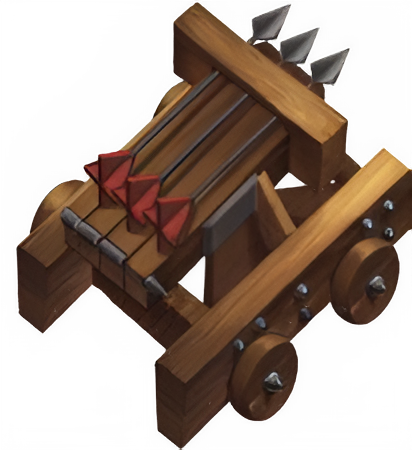
\includegraphics[width=0.1\paperwidth]{\_assets/ai/skill/skill_4.png}
    
\includegraphics[width=0.1\paperwidth]{\_assets/ai/skill/skill_5.png}
    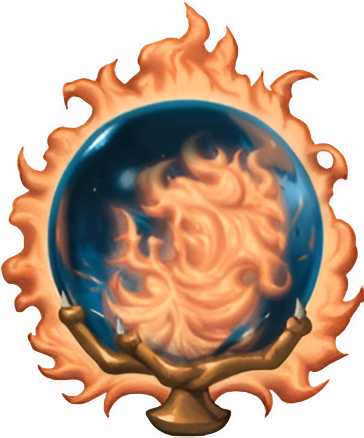
\includegraphics[width=0.1\paperwidth]{\_assets/ai/skill/skill_6.png}\\
    
\includegraphics[width=0.1\paperwidth]{\_assets/ai/skill/skill_7.png}
    
\includegraphics[width=0.1\paperwidth]{\_assets/ai/skill/skill_8.png}
    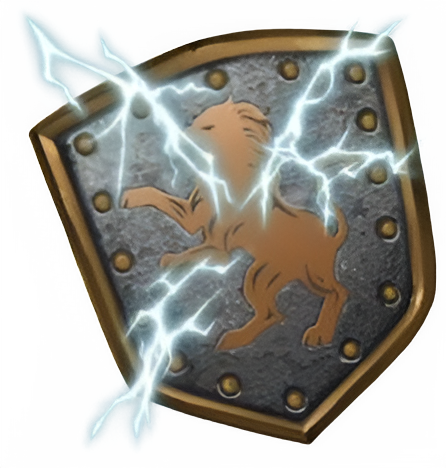
\includegraphics[width=0.1\paperwidth]{\_assets/ai/skill/skill_9.png}
    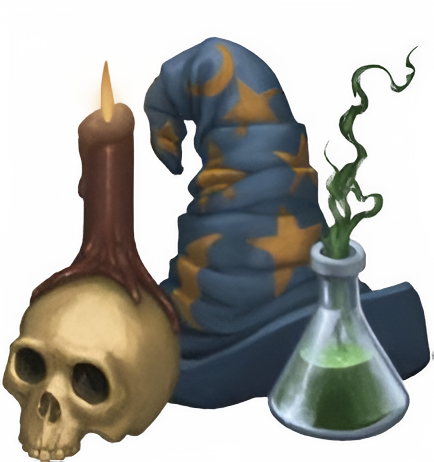
\includegraphics[width=0.1\paperwidth]{\_assets/ai/skill/skill_10.png}
    
\includegraphics[width=0.1\paperwidth]{\_assets/ai/skill/skill_11.png}
\end{center}

If you draw "Use a skill" and the ability AI deck is empty, shuffle this discard.

\newpage

\subsection*{\MakeUppercase{Spell list AI}}
When AI adds spells in his deck, draw cards until you draw one of the spell in the following lists, discard the other cards in the same order they were drawn: \\
\textbf{Air magic:} Chain lightning / Counterstrike / Disrupting Ray / Fortune / Haste / Lightning bolt / Precision.
\begin{center}
    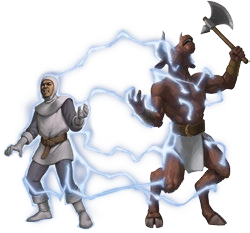
\includegraphics[width=0.1\paperwidth]{\_assets/ai/spell/air_spell_1.png}
    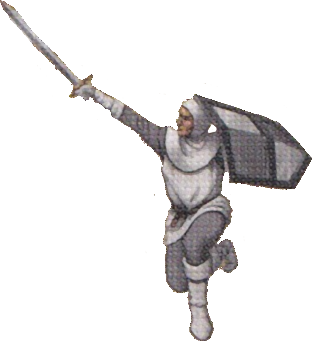
\includegraphics[width=0.1\paperwidth]{\_assets/ai/spell/air_spell_2.png}
    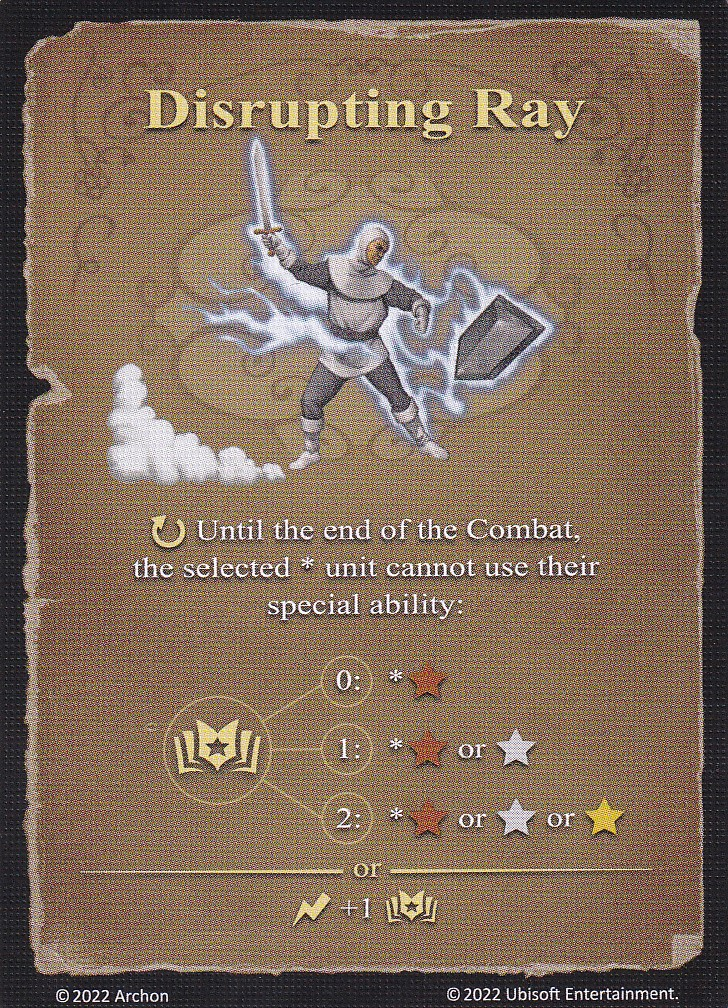
\includegraphics[width=0.1\paperwidth]{\_assets/ai/spell/air_spell_3.png}
    
\includegraphics[width=0.1\paperwidth]{\_assets/ai/spell/air_spell_4.png}
    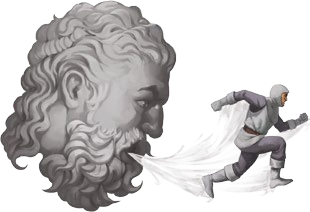
\includegraphics[width=0.1\paperwidth]{\_assets/ai/spell/air_spell_5.png}
    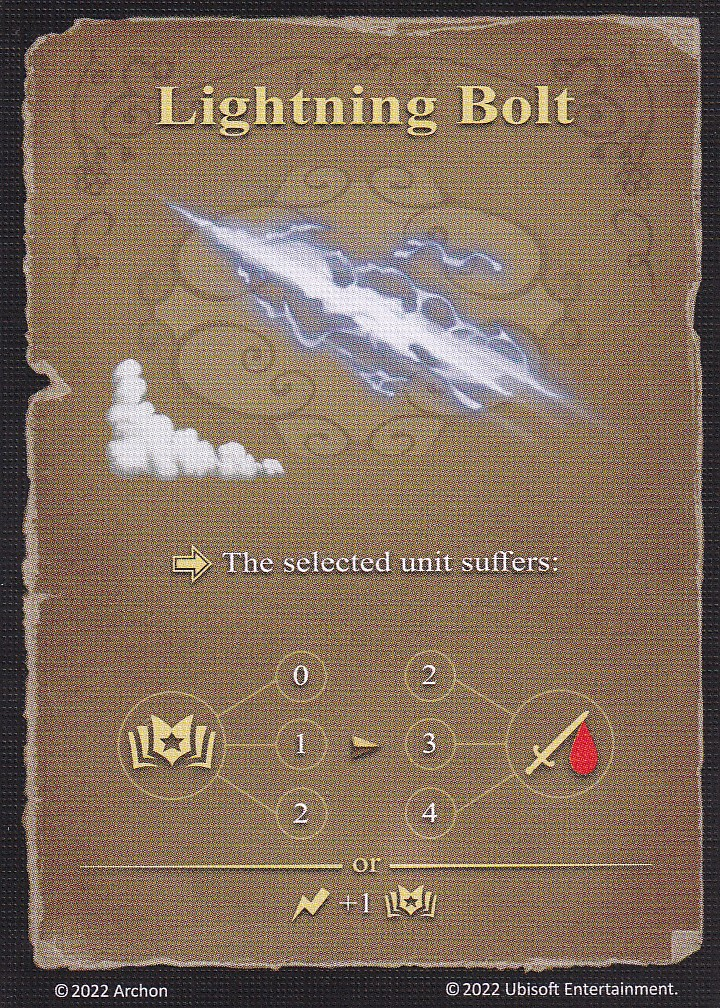
\includegraphics[width=0.1\paperwidth]{\_assets/ai/spell/air_spell_6.png}
    
\includegraphics[width=0.1\paperwidth]{\_assets/ai/spell/air_spell_7.png}
\end{center}

\textbf{Earth magic:} Anti-magic / Implosion / Resurrection / Shield / Slow / Sorrow / Stone skin.
\begin{center}
    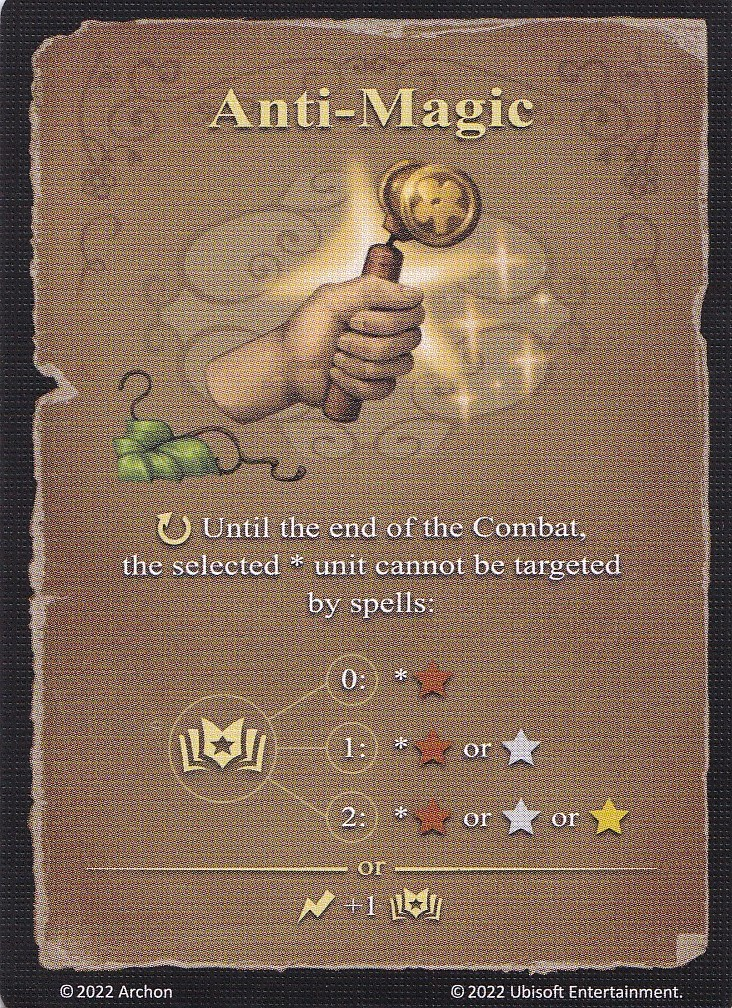
\includegraphics[width=0.1\paperwidth]{\_assets/ai/spell/earth_spell_1.png}
    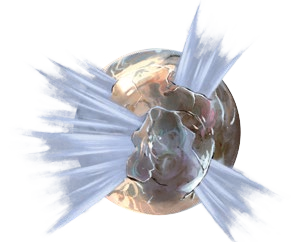
\includegraphics[width=0.1\paperwidth]{\_assets/ai/spell/earth_spell_2.png}
    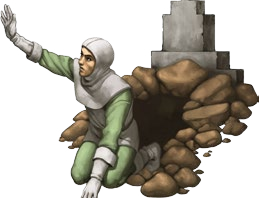
\includegraphics[width=0.1\paperwidth]{\_assets/ai/spell/earth_spell_3.png}
    
\includegraphics[width=0.1\paperwidth]{\_assets/ai/spell/earth_spell_4.png}
    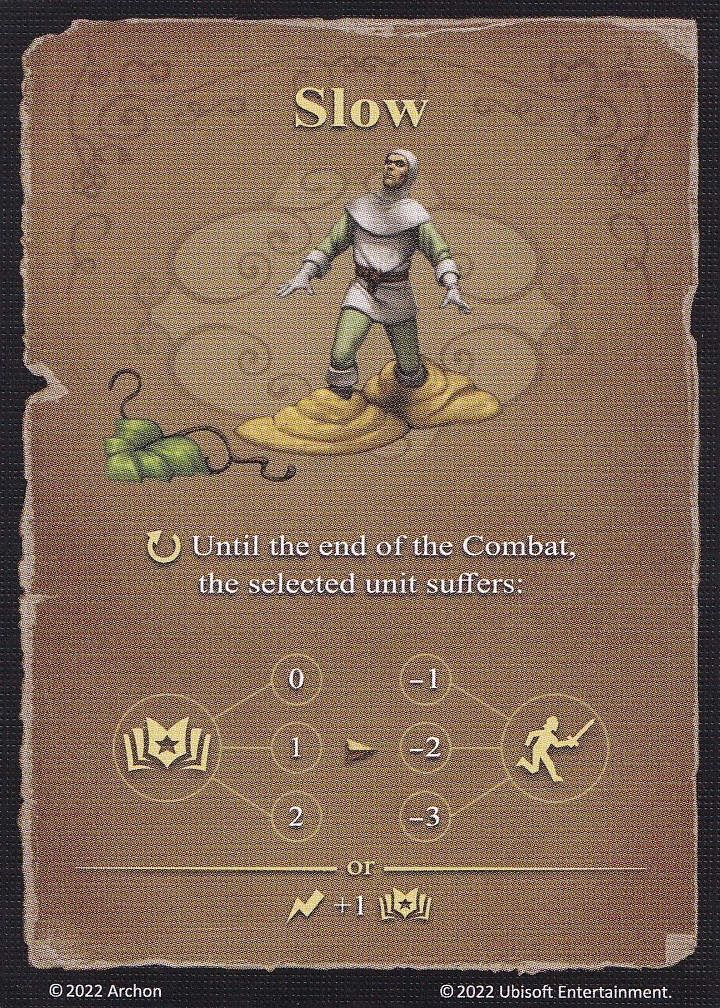
\includegraphics[width=0.1\paperwidth]{\_assets/ai/spell/earth_spell_5.png}
    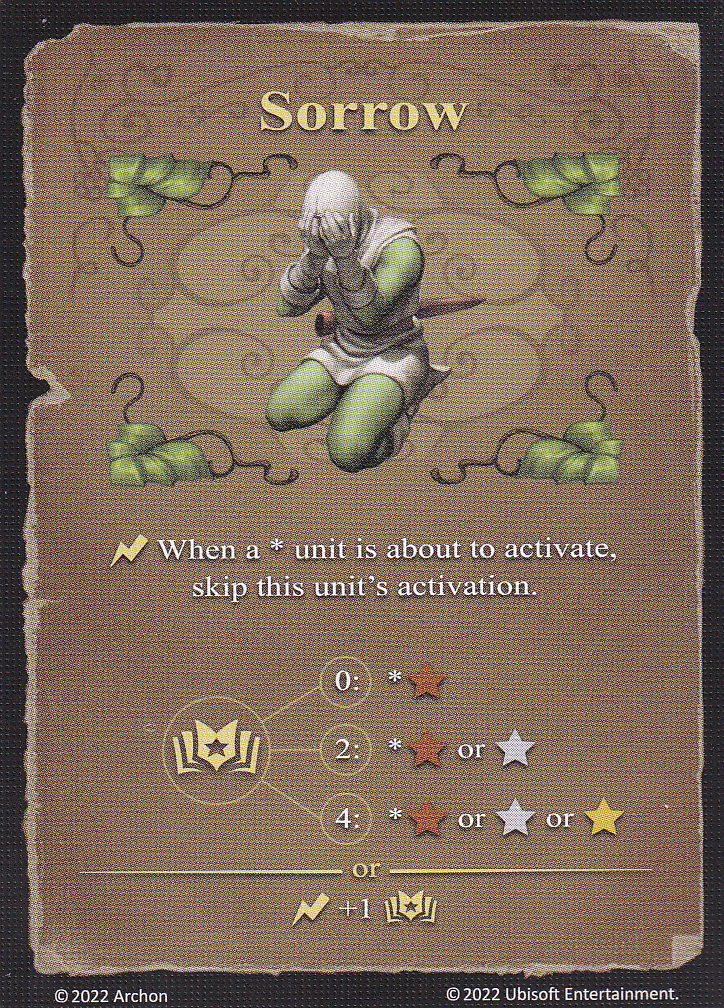
\includegraphics[width=0.1\paperwidth]{\_assets/ai/spell/earth_spell_6.png}
    
\includegraphics[width=0.1\paperwidth]{\_assets/ai/spell/earth_spell_7.png}
\end{center}

\textbf{Fire magic:} Berserk / Blind / Bloodlust / Curse / Fire shield / Frenzy / Misfortune / Slayer.
\begin{center}
    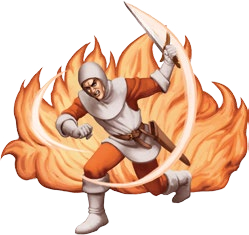
\includegraphics[width=0.1\paperwidth]{\_assets/ai/spell/fire_spell_1.png}
    
\includegraphics[width=0.1\paperwidth]{\_assets/ai/spell/fire_spell_2.png}
    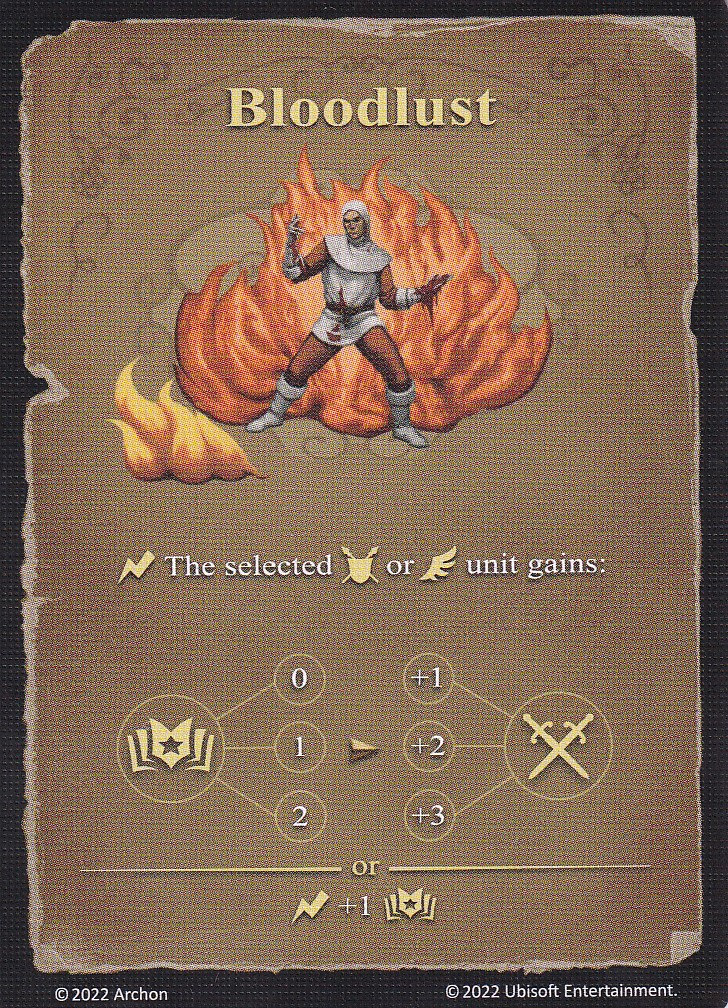
\includegraphics[width=0.1\paperwidth]{\_assets/ai/spell/fire_spell_3.png}
    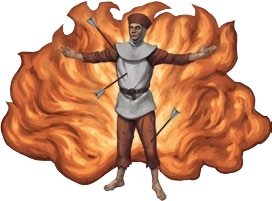
\includegraphics[width=0.1\paperwidth]{\_assets/ai/spell/fire_spell_4.png}
    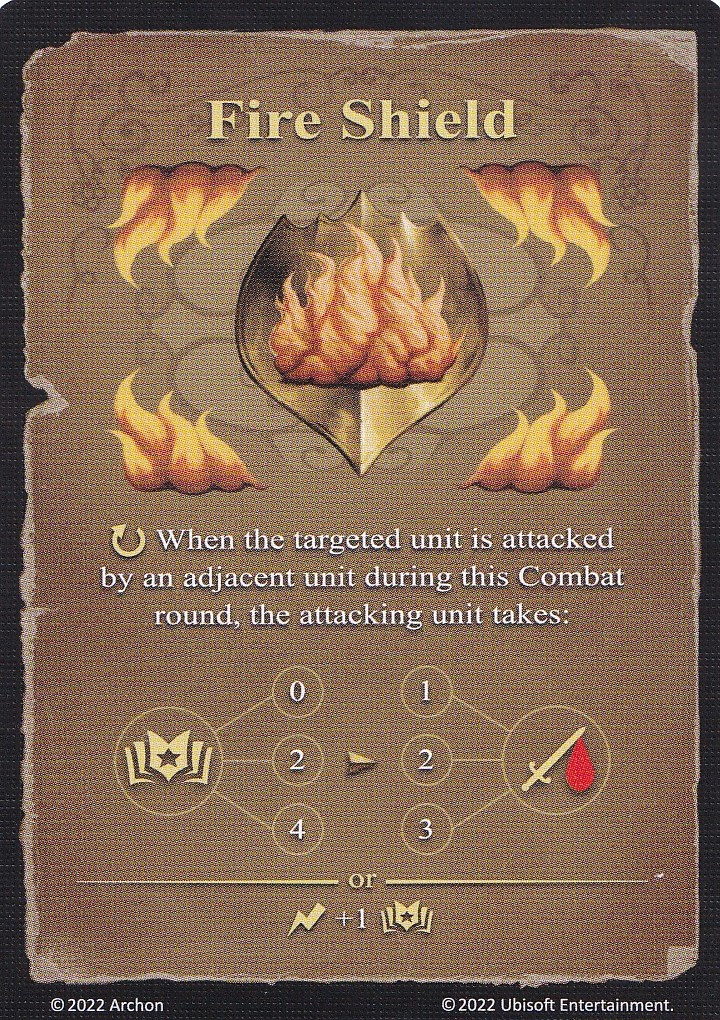
\includegraphics[width=0.1\paperwidth]{\_assets/ai/spell/fire_spell_5.png}
    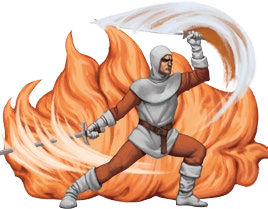
\includegraphics[width=0.1\paperwidth]{\_assets/ai/spell/fire_spell_6.png}
    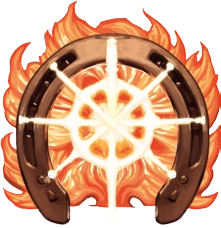
\includegraphics[width=0.1\paperwidth]{\_assets/ai/spell/fire_spell_7.png}
    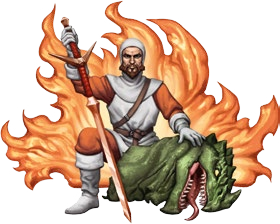
\includegraphics[width=0.1\paperwidth]{\_assets/ai/spell/fire_spell_8.png}
\end{center}

\textbf{Water magic:} Bless / Cure / Forgetfulness / Mirth / Weakness.
\begin{center}
    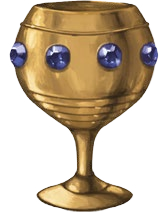
\includegraphics[width=0.1\paperwidth]{\_assets/ai/spell/water_spell_1.png}
    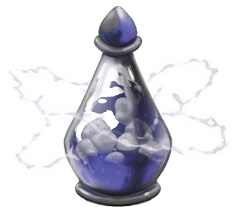
\includegraphics[width=0.1\paperwidth]{\_assets/ai/spell/water_spell_2.png}
    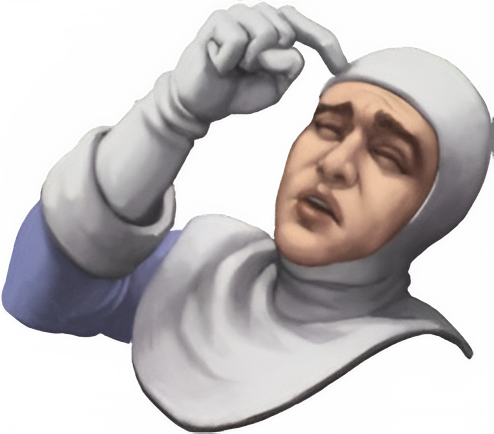
\includegraphics[width=0.1\paperwidth]{\_assets/ai/spell/water_spell_3.png}
    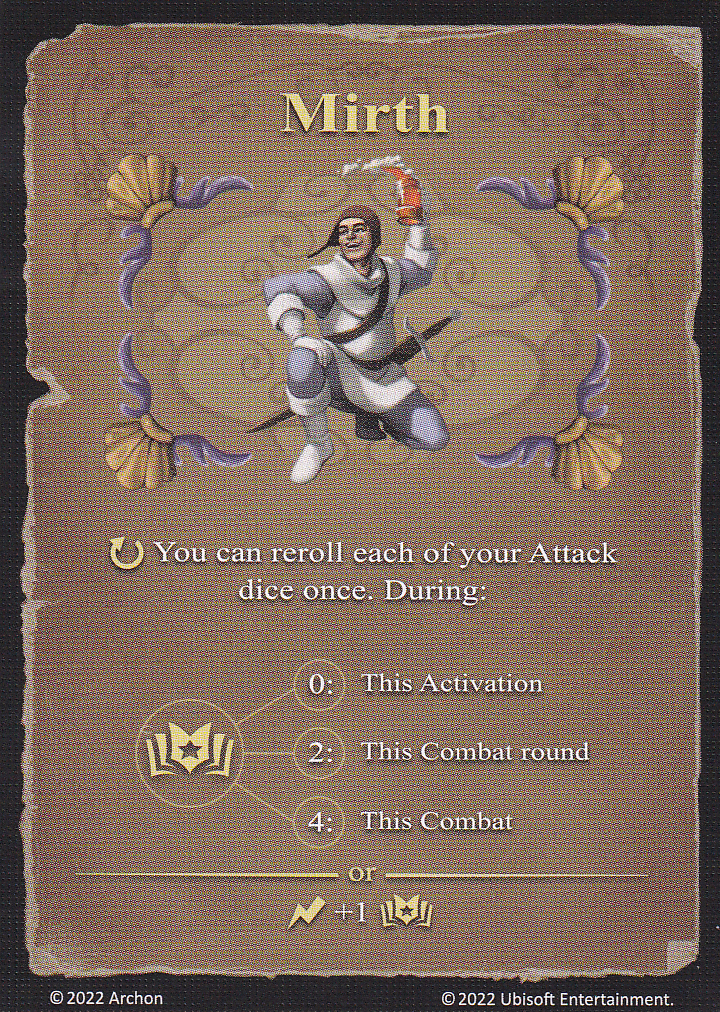
\includegraphics[width=0.1\paperwidth]{\_assets/ai/spell/water_spell_4.png}
    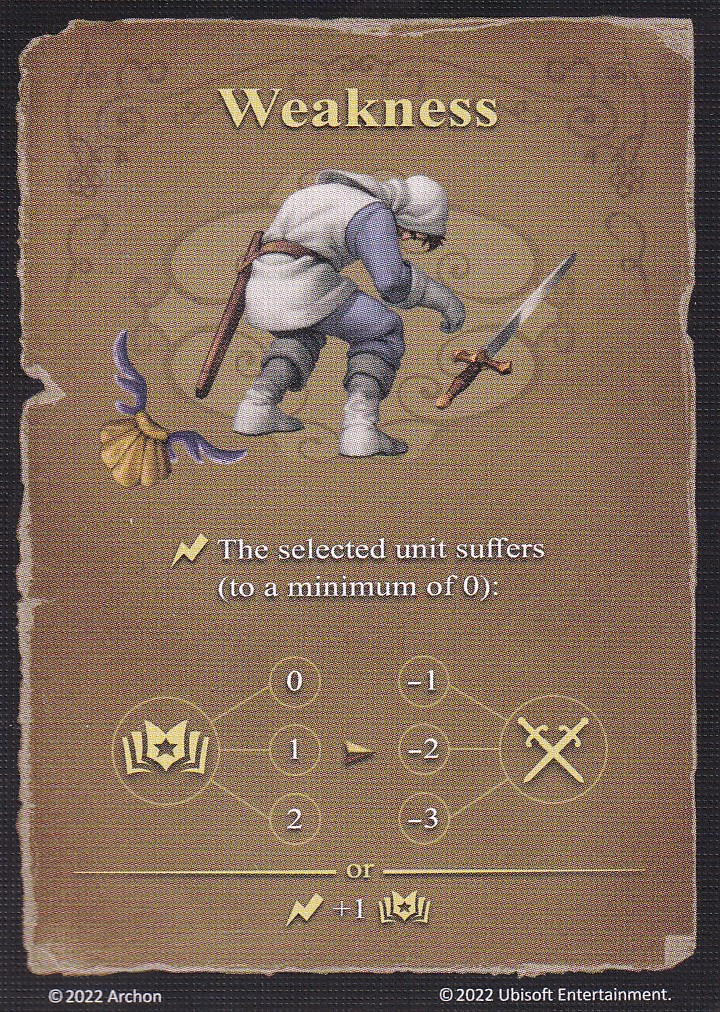
\includegraphics[width=0.1\paperwidth]{\_assets/ai/spell/water_spell_5.png}
\end{center}

\begin{multicols}{2}
    Or… Magic Arrow! 
    If you play in Impossible, AI can’t draw Magic Arrow, if you play in Easy, the AI can draw the earth spell Earthquake. \\ 
    If you draw "Cast a spell" and the spell AI deck is empty, shuffle this discard.
    \columnbreak
    \begin{center}
        
\includegraphics[width=0.1\paperwidth]{\_assets/ai/spell/magic_arrow.png}
        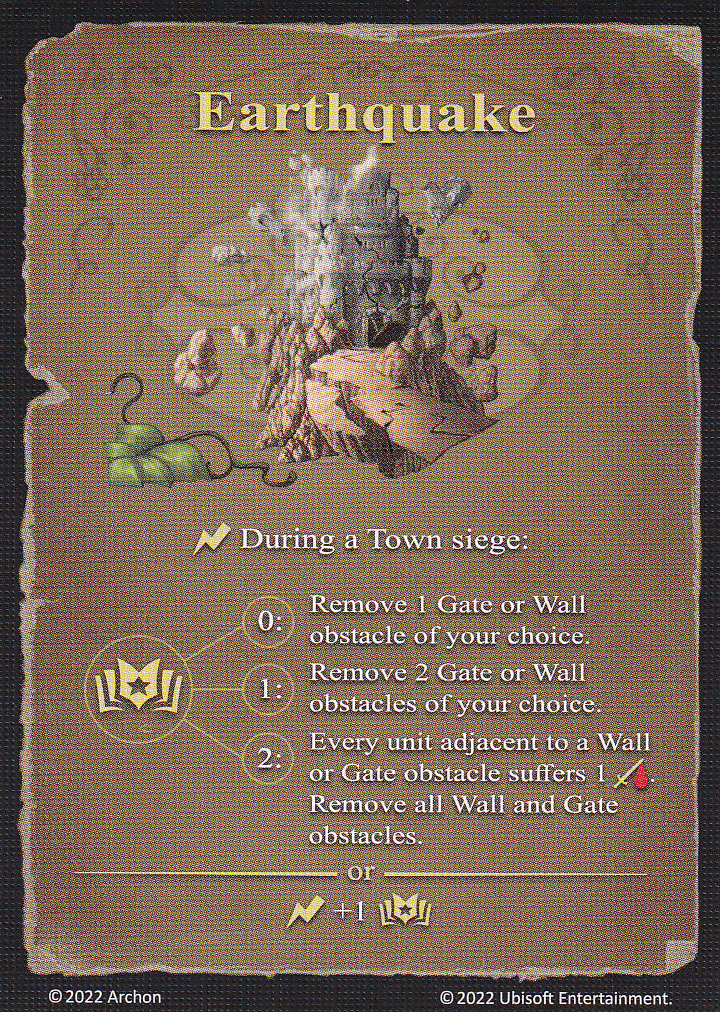
\includegraphics[width=0.1\paperwidth]{\_assets/ai/spell/earth_spell_8.png}
    \end{center}
\end{multicols}

\newpage

\subsection*{\MakeUppercase{F.A.Q.:}}

\begin{multicols}{2}
With all spells if the target is immune (like Efreet for fire magic or Titan for ongoing effects) or the spell has not enough power, choose the next eligible target. If a spell has enough power only to target bronze and there is no bronze in the army, discard it. The same goes for silver, if there is no silver or bronze in this army.

\begin{itemize}
    \item With \textbf{chain lightning}, the AI chooses the first target, but the player can choose the next target if tie.
    \item With \textbf{Counterstrike}, the AI can target only AI units with a black cube; if none (or not enough power) the spell is discarded.
    \item With \textbf{Fortune}, the AI rolls and chooses in order +1 then 0 then -1.
    \item With \textbf{Precision}, the AI can target only ranged AI units, if none (or not enough power) discard the spell.
    \item With \textbf{resurrection} / \textbf{Frenzy} / \textbf{Slayer} / \textbf{Shield} / \textbf{Sorrow} / \textbf{Stone skin}, keep the card next to the battlefield with black cubes as reminder of the power of the spell, the AI cast this spell only when the conditions are right: 
    \begin{itemize}
        \item For \textbf{resurrection}, when AI unit is killed.
        \item For \textbf{stone skin} / \textbf{Shield} when AI unit is attacked.
        \item For \textbf{Slayer}, when AI unit attacked a gold unit.
        \item For \textbf{Frenzy}, when AI unit attacked a unit the spell can affect (even if this unit has already 0 shield).
        \item For \textbf{sorrow}, when a player unit start their turn.
    \end{itemize}
    \item With \textbf{Cure}, the AI can target only AI units with at least one damage token, if none (or not enough power) discard the spell.
    \item With \textbf{Forgetfulness}, the AI can target only ranged player units, if none (or not enough power) discard the spell. 
    \item With \textbf{Mirth}, AI rerolls only -1 dice.
    \item With \textbf{Earthquake}, AI chooses gate at first, if gate are already destroyed, the player chooses which wall is destroyed.
\end{itemize}

\begin{itemize}
    \item With \textbf{Armorer}/ \textbf{Resistance} / \textbf{Sorcery}, keep the card next to the battlefield, the AI cast this ability only when the conditions are right:
    \begin{itemize}
        \item For \textbf{Armorer}, when AI unit is attacked.
        \item For \textbf{Sorcery}, when the next spell is cast.
        \item For \textbf{Resistance}, the next time the player casts a spell with 0 or 1 power, the AI cancels this spell (don’t forget in impossible, the card is played twice, put two black cubes on the card, after the first player's spell, remove one cube, after the second remove this card).
    \end{itemize}
    \item With \textbf{First aid}, the AI can target only AI units with at least one damage token, if none discard the ability. 
    \item With \textbf{Air magic} / \textbf{Earth magic} / \textbf{Fire magic} / \textbf{Water Magic}, keep it in the AI ability deck until a "use a skill" is played by the AI and draws this, then if there is already another permanent card, discard the old one and play the new one. In impossible he only  plays this card once.
\end{itemize}
\end{multicols}


\newpage

\hommtable{38}{
    \centering
    \textbf{Optional Rules Table}\\
    
    \small
    {
        \color{white}
        You may modify the rules of AI to increase or decrease the game's difficulty.\\
    }
    \bigskip
    
    \begin{tabularx}{\linewidth}{>{\hsize=0.3\hsize\linewidth=\hsize}X
            >{\hsize=1.7\hsize\linewidth=\hsize}X}
        \darkcell[1.5]{\color{white}Game Difficulty Levels} & \darkcell[1.5]{Change to the default rules} \\
        \darkcell[1.2]{Increase} & \lightcell[1.2]{If AI draw ability Air magic or Earth magic or Fire magic or Water Magic, the spell list it can draw from are reduced to only magic arrow and the spells of this element(s).} \\
        \darkcell[1.2]{Increase} & \lightcell[1.2]{If AI draws ability Air magic or Earth magic or Fire magic or Water Magic, he cannot add another permanent card.} \\
        \darkcell[0.8]{Increase} & \lightcell[0.8]{AI progress is advanced by one turn.} \\
        \darkcell[0.8]{Decrease} & \lightcell[0.8]{AI progress is delayed by one turn.} \\
        \darkcell[0.8]{Decrease} & \lightcell[0.8]{The AI can only use magic arrow.} \\
        \darkcell[0.8]{Decrease} & \lightcell[0.8]{The AI can reinforce but has no wall/gate/tower with him if fight is in his town.} \\
        \darkcell[1.2]{Decrease} & \lightcell[1.2]{AI can only use half (round up) of its AI Hero cards.} \\
        \darkcell[1.2]{Decrease} & \lightcell[1.2]{AI can use only 4 units (remove the weakest in the list (in the majority of cases : few bronze)).} \\
        \darkcell[1.2]{Variant} & \lightcell[1.2]{In multiplayer, players fight against the same AI unit deck (recreate the deck for each player).} \\
        \darkcell[0.8]{Variant} & \lightcell[0.8]{In multiplayer, the AI uses the same spell deck and ability deck against all players (don’t forget to shuffle it at start of battle).} \\
        \darkcell[0.8]{Variant} & \lightcell[0.8]{The AI can only use one spell (draw this in spell list at start of game).} \\
        \darkcell[0.8]{Variant} & \lightcell[0.8]{The AI can only use one ability (draw this in ability list at start of game).} \\
    \end{tabularx}
}
